\section{Aufbau \cite{sample}}

\begin{figure}
  \centering
  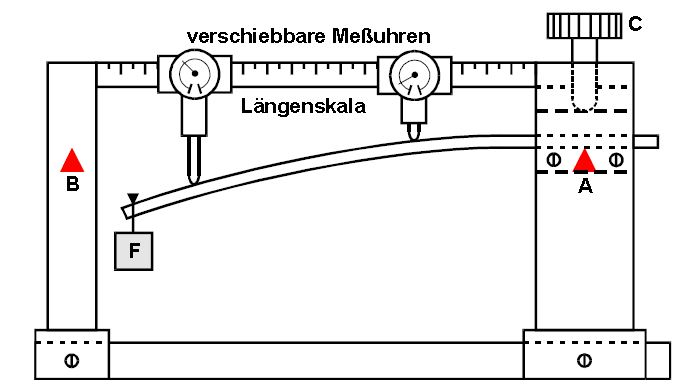
\includegraphics[width=\textwidth]{Text/Aufbau.jpg}
  \caption{Helmholz-Spulenpaar \cite[2]{sample}}
  \label{fig:aufbau}
\end{figure}

Ein kleiner zylindrischer Permanentmagnet befindet sich in der Mitte von einer Billardkugel.
Das magnetische Moment $\mu_{\symup{Dipol}}$ des Permanentmagneten zeigt in Richtung des Stiels.
Das homogene Magnetfeld wird durch ein Helmholtz-Spulenpaar,
mit den Abmessungen $N = 195$, $d = 0,138 \mathrm{m}$ und $R = 0,109 \mathrm{m}$, erzeugt.
In der Mitte der Anordnung befindet sich ein Messingzylinder mit einem Luftkissen
und an der oberen Spule befindet sich ein Stroboskop zur Bestimmung der Drehbewegung.
